% Section 1: Introduction to Classification (Slides 1-6)

% Slide 1: Title Slide
\begin{frame}[plain]
  \vspace{0.4cm}
  \begin{center}
    {\fontsize{8}{10}\selectfont\color{subgray}دانشگاه مانهایم \ | \ گروه علوم داده و وب}\\[0.35cm]
    {\fontsize{20}{24}\selectfont\color{mannheimblue}\textbf{طبقه‌بندی داده‌ها (بخش ۱)}}\\[0.25cm]
    {\fontsize{13}{16}\selectfont\color{subgray}\textbf{\lr{IE500} داده‌کاوی}}\\[0.45cm]
    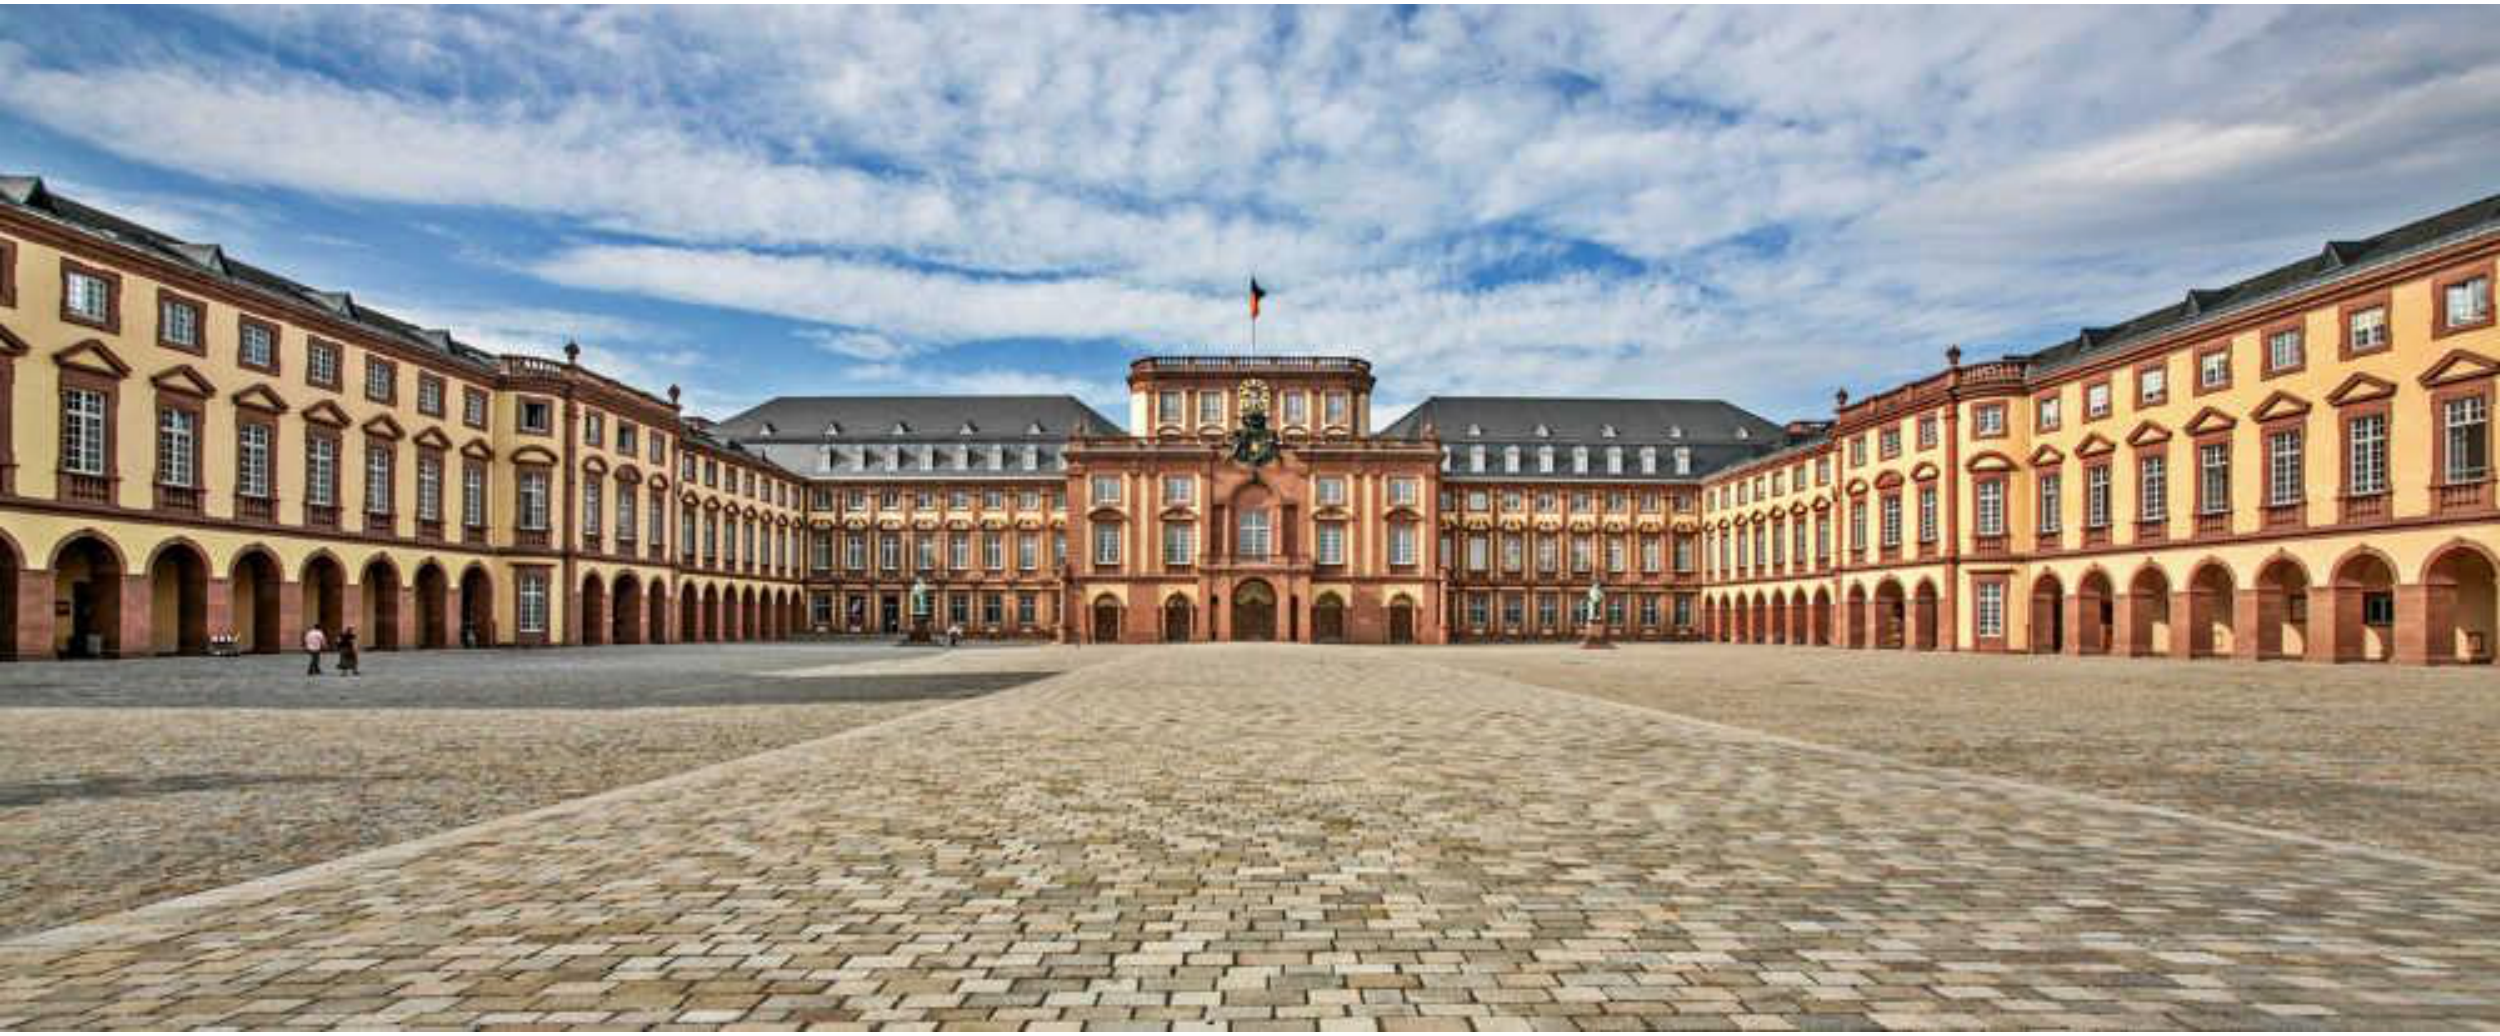
\includegraphics[width=\textwidth,height=4.1cm,keepaspectratio]{images/page_01_img_1.png}\\[0.3cm]
    {\fontsize{7.5}{9}\selectfont\color{subgray}نسخه \lr{16.09.2024}}
  \end{center}
\end{frame}

% Slide 2: Outline
\begin{frame}{سرفصل مطالب}
  \begin{itemize}
    \setlength{\itemsep}{14pt}
    \item \textbf{درخت‌های تصمیم (\lr{Decision Trees})}
    \begin{itemize}
      \item ساختار درخت، مرزهای تصمیم، الگوریتم هانت و روش‌های تفکیک
    \end{itemize}
    \item \textbf{معیار خلوص جینی (\lr{Gini Impurity Index})}
    \begin{itemize}
      \item فرمول ریاضی، نحوه محاسبه برای ویژگی‌های اسمی، ترتیبی و پیوسته
    \end{itemize}
    \item \textbf{پدیده بیش‌برازش (\lr{Overfitting})}
    \begin{itemize}
      \item علل، نشانه‌ها، تیغ اوکام و راهکارهای پیشگیری (هرس اولیه و یادگیری جمعی)
    \end{itemize}
    \item \textbf{الگوریتم‌های یادگیری جمعی (\lr{Ensembles})}
    \begin{itemize}
      \item جنگل‌های تصادفی (\lr{Random Forest}) و \lr{XGBoost}
    \end{itemize}
    \item \textbf{معیارهای ارزیابی مدل (\lr{Evaluation Metrics})}
    \begin{itemize}
      \item ماتریس درهم‌ریختگی، صحت، دقت، بازخوانی، معیار \lr{F1}، ارزیابی هزینه‌محور و منحنی‌های \lr{ROC}
    \end{itemize}
  \end{itemize}
\end{frame}

% Slide 3: Introduction to Classification
\begin{frame}{مقدمه‌ای بر طبقه‌بندی داده‌ها}{تعریف هدف اصلی}
  \begin{itemize}
    \item \textbf{هدف اصلی:} یادگیری یک مدل برای تشخیص و شناسایی یک مفهوم (برای نمونه: «درخت»)
  \end{itemize}
  \vspace{0.2cm}
  \begin{center}
    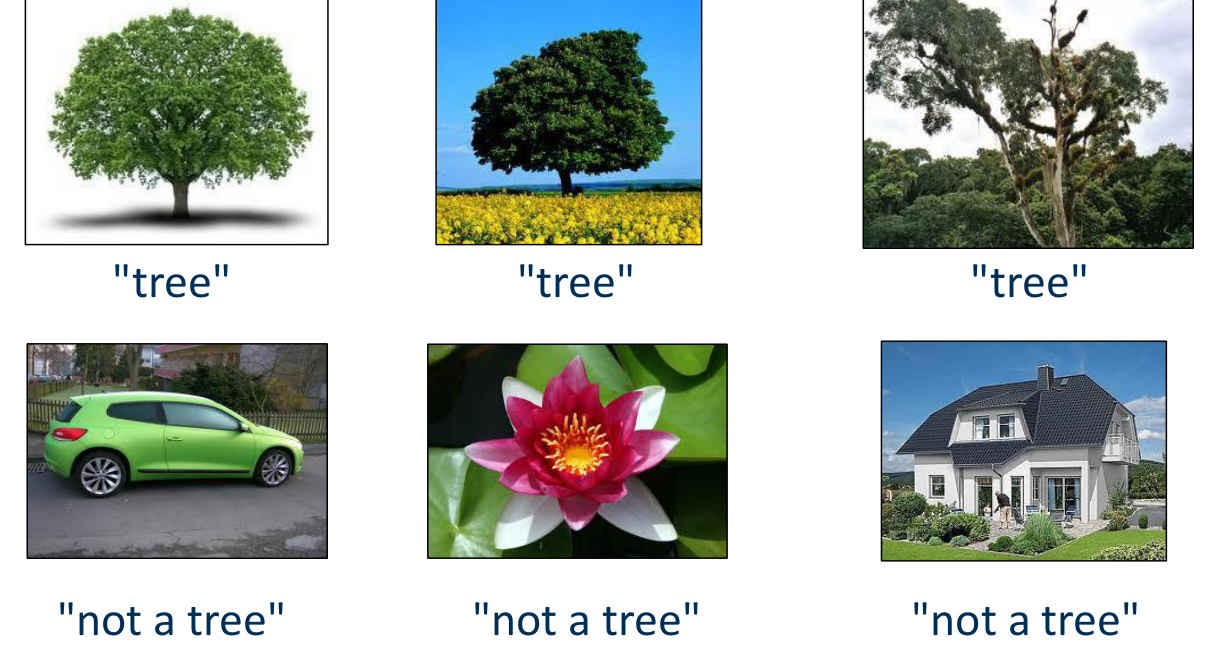
\includegraphics[width=0.92\textwidth,height=5.2cm,keepaspectratio]{images/slide03_concept_examples_clean.png}
  \end{center}
\end{frame}

% Slide 4: Learning a Concept
\begin{frame}{مقدمه‌ای بر طبقه‌بندی}{یادگیری مفهوم و چالش‌های تعمیم}
  \begin{columns}[c]
    \begin{column}{0.62\textwidth}
      \begin{itemize}
        \setlength{\itemsep}{3pt}
        \item \textbf{مثال: یادگیری یک مفهوم جدید، مثلاً «درخت»}
        \begin{itemize}
          \setlength{\itemsep}{2pt}
          \item مشاهده نمونه‌های مثبت و منفی (داده‌های آموزش \lr{Training data})
          \item استخراج یک مدل؛ برای مثال: «درختان، گیاهان بزرگ و سبزرنگی هستند»
        \end{itemize}
      \end{itemize}
    \end{column}
    \begin{column}{0.36\textwidth}
      \centering
      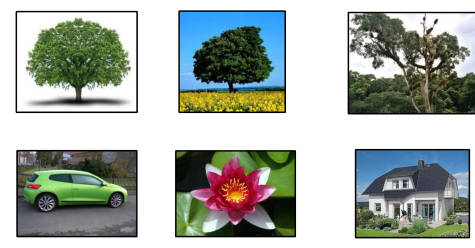
\includegraphics[width=\textwidth]{images/slide04_train_samples.png}
    \end{column}
  \end{columns}
  \vspace{0.15cm}
  \begin{itemize}
    \item \textbf{هدف: طبقه‌بندی نمونه‌های ندیده و جدید (\lr{Unseen instances})}
  \end{itemize}
  \vspace{0.05cm}
  \centering
  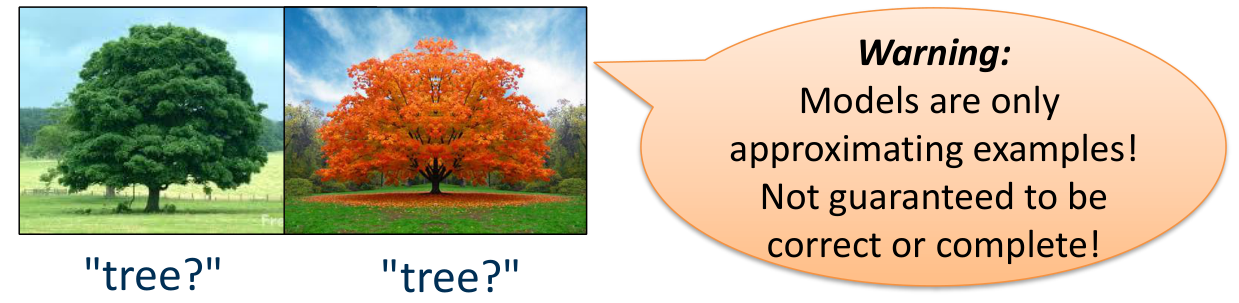
\includegraphics[width=0.90\textwidth,height=2.5cm,keepaspectratio]{images/slide04_bottom_graphics.png}
\end{frame}

% Slide 5: The Classification Workflow
\begin{frame}{گردش کار طبقه‌بندی داده‌ها}{چرخه کامل یادگیری و ارزیابی}
  \begin{center}
    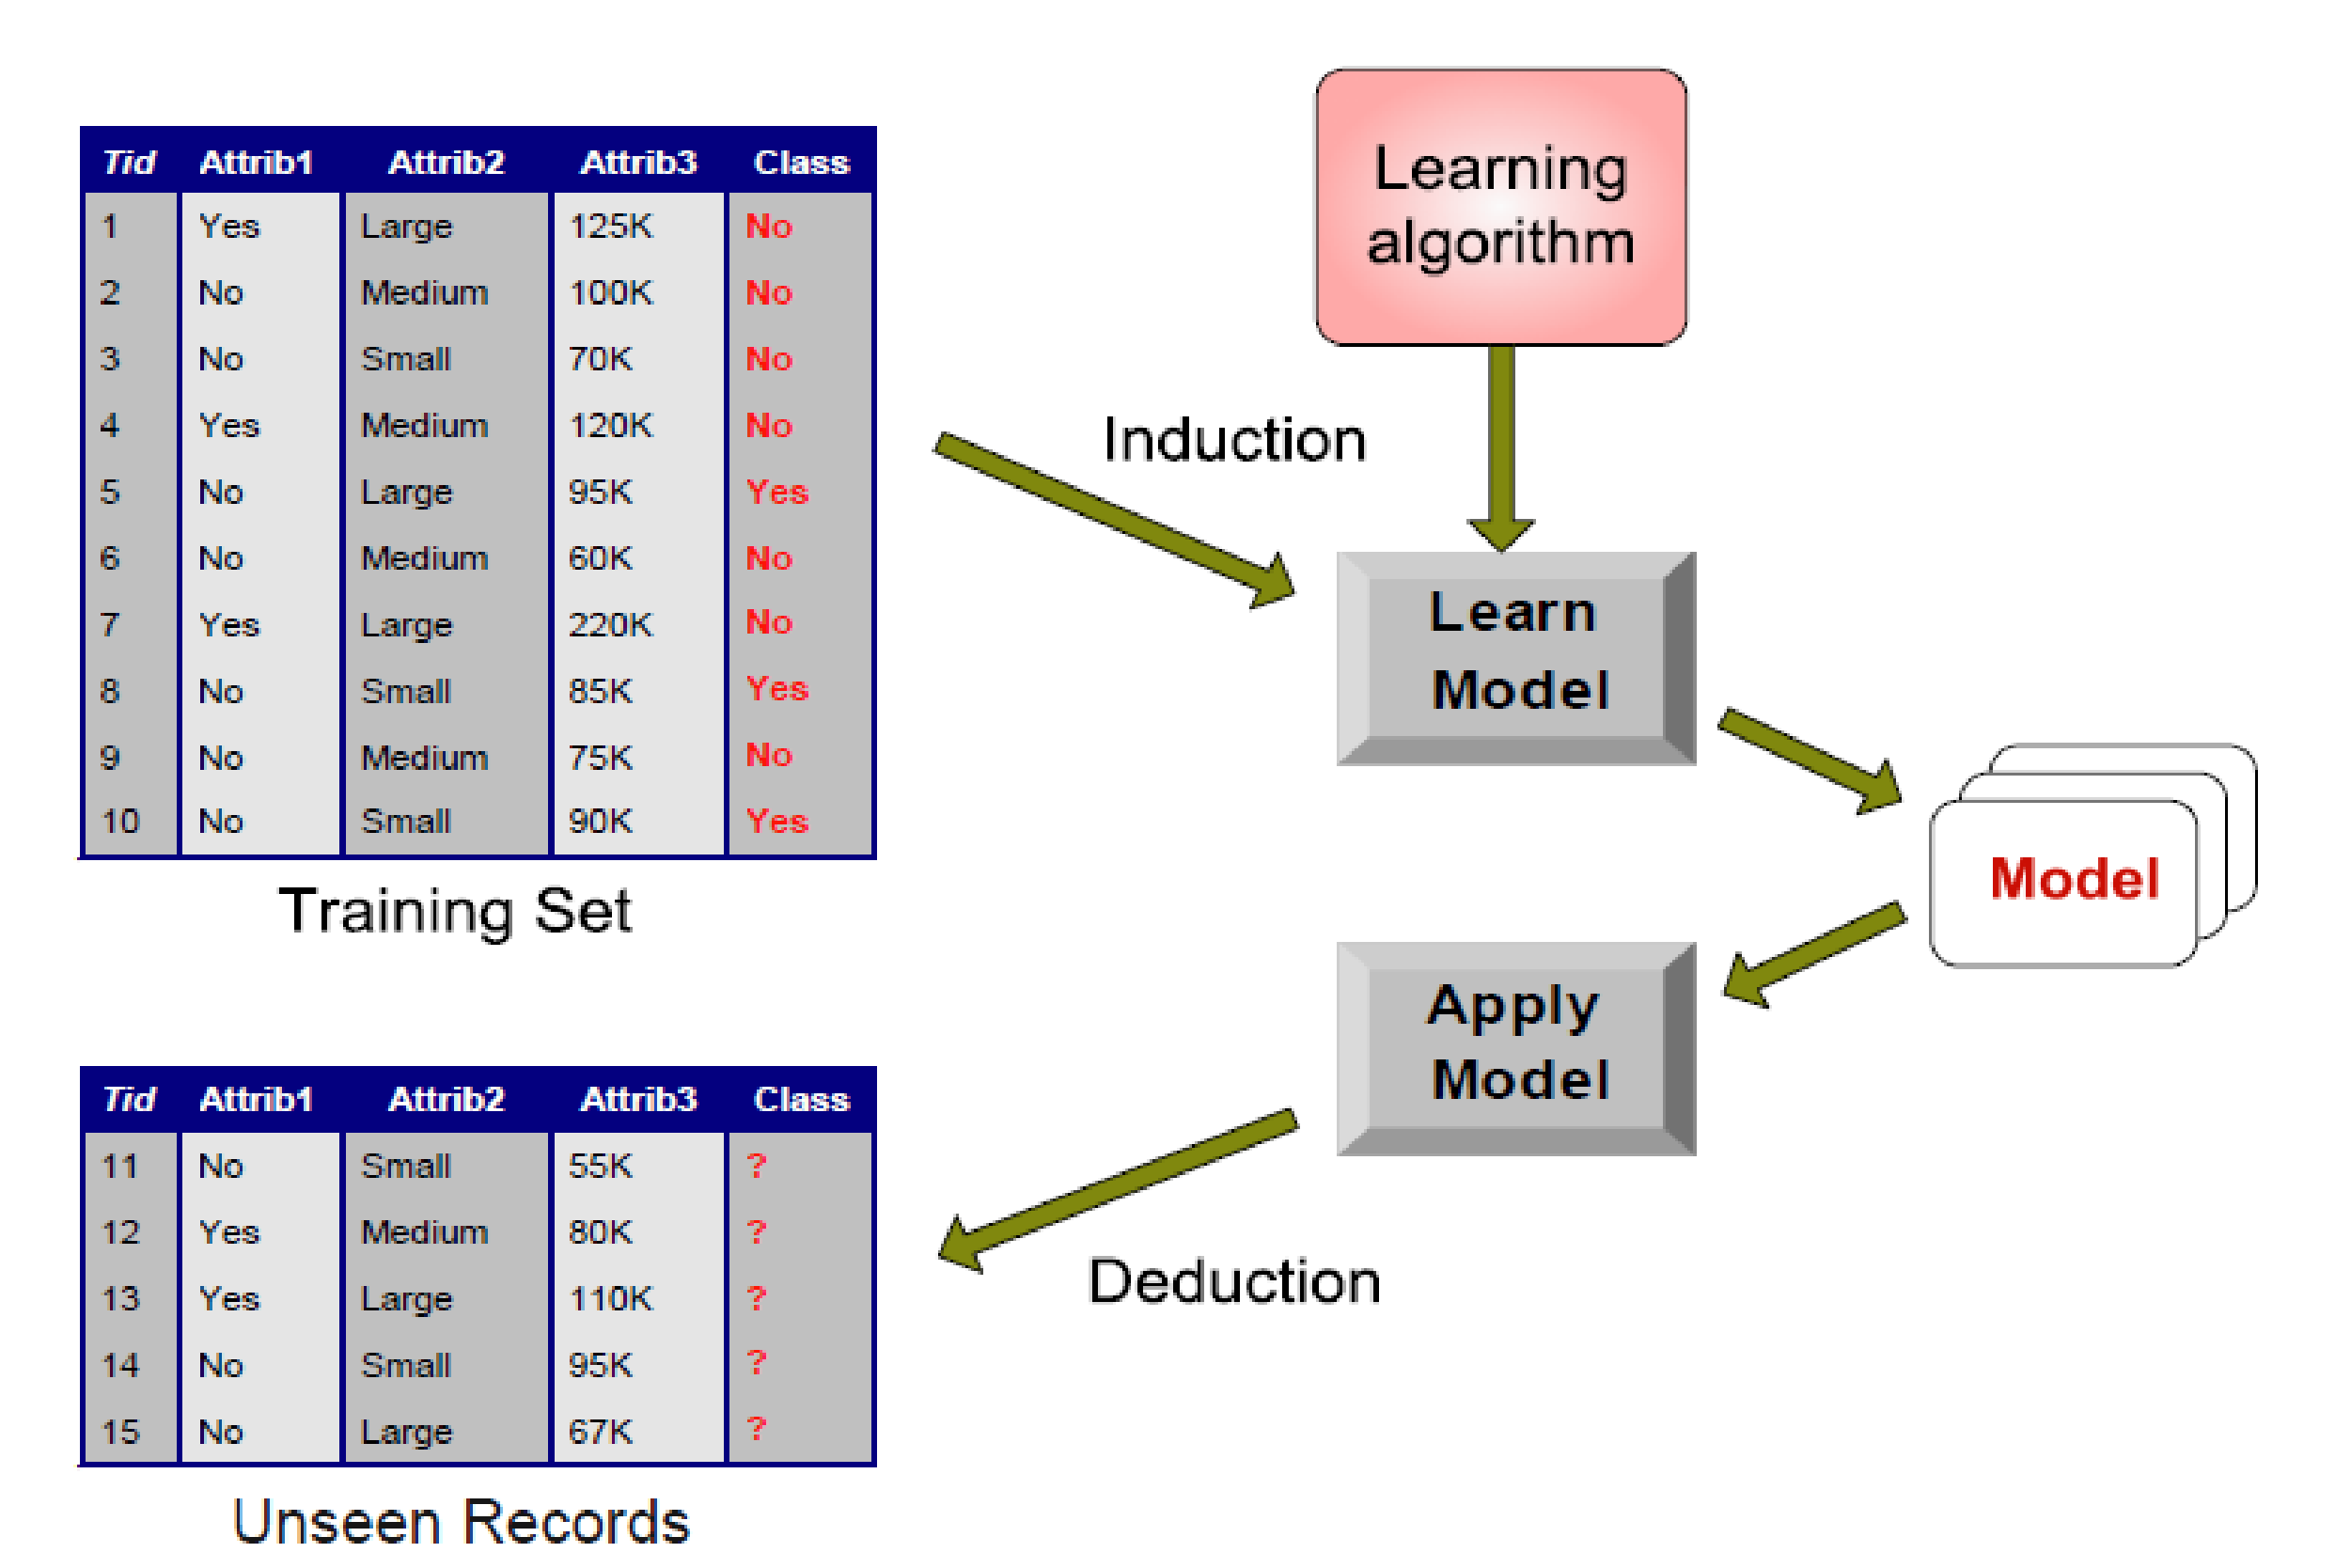
\includegraphics[width=0.96\textwidth,height=5.8cm,keepaspectratio]{images/slide05_workflow.png}
  \end{center}
\end{frame}

% Slide 6: Lazy vs Eager Learning
\begin{frame}{یادگیری تنبل در برابر یادگیری مشتاق}{\lr{Lazy vs. Eager Learning}}
  \begin{itemize}
    \setlength{\itemsep}{10pt}
    \item \textbf{یادگیری تنبل:} \lr{(Lazy Learning)}
    \begin{itemize}
      \setlength{\itemsep}{3pt}
      \item روش‌های مبتنی بر نمونه (\lr{Instance-based}) مانند الگوریتم \lr{k-NN}
      \item هیچ مدلی را از پیش به صورت صریح استخراج و ذخیره نمی‌کنند.
      \item فرآیند «یادگیری» و محاسبات تنها در زمان تقاضا برای طبقه‌بندی یک رکورد جدید انجام می‌شود.
      \item \textbf{تک‌هدف:} پیش‌بینی برچسب رکوردهای جدید با حداکثر دقت ممکن.
    \end{itemize}
    \item \textbf{یادگیری مشتاق:} \lr{(Eager Learning)}
    \begin{itemize}
      \setlength{\itemsep}{3pt}
      \item یک مدل صریح و ساختاریافته پیش از رسیدن داده‌های جدید ساخته می‌شود.
      \item \textbf{دو هدف اساسی:}
      \begin{enumerate}
        \setlength{\itemsep}{2pt}
        \item طبقه‌بندی دقیق رکوردهای نامشاهده‌شده و جدید
        \item درک و تحلیل ساختار حوزه کاربرد به شکلی قابل‌تفسیر برای انسان (\lr{Explainable AI})
      \end{enumerate}
      \item \textbf{نمونه‌های بارز:} درخت‌های تصمیم (\lr{Decision Trees})، رگرسیون لجستیک
    \end{itemize}
  \end{itemize}
\end{frame}
